%iffalse
\let\negmedspace\undefined
\let\negthickspace\undefined
\documentclass[journal,12pt,onecolumn]{IEEEtran}
\usepackage{cite}
\usepackage{amsmath,amssymb,amsfonts,amsthm}
\usepackage{algorithmic}
\usepackage{graphicx}
\usepackage{textcomp}
\usepackage{xcolor}
\usepackage{txfonts}
\usepackage{listings}
\usepackage{enumitem}
\usepackage{mathtools}
\usepackage{gensymb}
\usepackage{comment}
\usepackage[breaklinks=true]{hyperref}
\usepackage{tkz-euclide} 
\usepackage{gvv}                                        
%\def\inputGnumericTable{}                                 
\usepackage[latin1]{inputenc}     
\usepackage{xparse}
\usepackage{color}                                            
\usepackage{array}                                            
\usepackage{longtable}                                       
\usepackage{calc}                                             
\usepackage{multirow}
\usepackage{multicol}
\usepackage{hhline}                                           
\usepackage{ifthen}                                           
\usepackage{lscape}
\usepackage{tabularx}
\usepackage{array}
\usepackage{float}
\newtheorem{theorem}{Theorem}[section]
\newtheorem{problem}{Problem}
\newtheorem{proposition}{Proposition}[section]
\newtheorem{lemma}{Lemma}[section]
\newtheorem{corollary}[theorem]{Corollary}
\newtheorem{example}{Example}[section]
\newtheorem{definition}[problem]{Definition}
\newcommand{\BEQA}{\begin{eqnarray}}
\newcommand{\EEQA}{\end{eqnarray}}
\newcommand{\define}{\stackrel{\triangle}{=}}
\theoremstyle{remark}
\newtheorem{rem}{Remark}
% Marks the beginning of the document
\begin{document}
\title{AR:ARCHITECTURE AND PLANNING}
\author{AI25btech11027 - Bhuvana}
\maketitle
\renewcommand{\thefigure}{\theenumi}
\renewcommand{\thetable}{\theenumi}
\begin {center}
\large \textbf{2019}\\
\end{center}
\textbf{Q.1 to Q.10 carry one mark each}
\begin{enumerate}
\item The fishermen, \underline{\makebox[2cm]{\hfill}} the flood victims owed their lives, were rewarded by the government \hfill \textbf{(GATE EE 2025)}
\begin{enumerate}
    \begin{multicols}{4}
    \item whom
    \item to which
    \item to whom
    \item that
    \end{multicols}
    \end{enumerate}
\item Some students were not involved in the strike.\hfill \textbf{(GATE EE 2025)}\\
If the above statement is true which of the following conclusions is/are logically necessary?\\
1. some who were involved in the strike were students.\\
2. No student was involved in the strike.\\
3. At least one student was involved in the strike.\\
4. Some who were not involved in the strike were students.\\
\begin{enumerate}
    \begin{multicols}{4}
        \item 1 and 2
        \item 3
        \item 4
        \item 2 and 3
    \end{multicols}
\end{enumerate}
\item The radius as well as the height of a circular cone increases by $10\%$.The percentage increase in its volume is \underline{\makebox[2cm]{\hfill}} \hfill \textbf{(GATE EE 2025)}
\begin{enumerate}
    \begin{multicols}{4}
        \item $17.1$
        \item $21.0$
        \item $33.1$
        \item $72.8$
    \end{multicols}
\end{enumerate}
\item Five numbers $10,7,5,4 $ and $2$ are to be arranged in a sequence from left to right following the direcions given below: \hfill \textbf{(GATE EE 2025)}\\
1. No two odd or even numbers are next to each other.\\
2. The second number from the left is exactly half of the left-most number.\\
3. The middle number is exactly twice the right-most number.\\
Which is the second number from the right?
\begin{enumerate}
    \begin{multicols}{4}
        \item 2
        \item 4
        \item 7
        \item 10
    \end{multicols}
\end{enumerate}
\item Until Iran came along,India had never been \underline{\makebox[2cm]{\hfill}} in kabaddi. \hfill \textbf{(GATE EE 2025)}
\begin{enumerate}
    \begin{multicols}{4}
        \item defeated
        \item defeating
        \item defeat
        \item defeatist
    \end{multicols}
\end{enumerate}
\textbf{Q.6 to Q.10 carry two marks each}
\item Since the last one year,after a 125 basis point reduction in repo by the Reserve Bank of India,banking institutions have been making a demand to reduce interest rates on small saving schemes.Finally,the government announced yesterday a reduction in interest rates on small saving schemes to bring them on par with fixed deposit interest rates.\\
Which one of the following statements can be inferred from the given passage? \hfill \textbf{(GATE EE 2025)}
\begin{enumerate}
    \item Whenever the Reserve Bank of India reduces the repo rate ,the interest rates on small saving schemes are also reduced
    \item Interest rates on small saving schemes are always maintained on par with fixed deposit interest rates.
    \item The government sometimes takes into consideration the demands of banking institutions before reducing the interest rates on small saving schemes
    \item A reduction in interest rates on small saving schemes follow only after  a reduction in repo rate by the Reserve Bank of India
\end{enumerate}
\item In a country of 1400 millions population,$70\%$ own mobile phones. Among these Internet users,only half buy goods from e-commerce portals. What is the percentage of these buyers in the country? \hfill \textbf{(GATE EE 2025)}
\begin{enumerate}
    \begin{multicols}{4}
        \item $10.50$
        \item $14.70$
        \item $15.00$
        \item $50.00$
    \end{multicols}
\end{enumerate}
\item The nomenclature of Hindustani music has changed over the centuries.Since the medieval period \textit{dhrupad} styles were identified as \textit{baanis}. Terms like \textit{gaayaki} and \textit{baaj} were used to refer to vocal and instumental styles,respectively. With the institutionalization of music education the term \textit{gharana} became acceptable.\textit{gharana} originally referred to hereditary musicians from a particular lineage,including disciples and grand disciples.\\
Which one of the following pairings is \textbf{NOT} correct? \hfill \textbf{(GATE EE 2025)}
\begin{enumerate}
        \item \textit{dhrupad,baani}
        \item \textit{gayaki},vocal
        \item \textit{baaj},institution
        \item \textit{gharana},lineage
\end{enumerate}
\item Two trains started at 7AM from the same point. The first train travelled north at a speed of $80 \text{km/h}$ and the second train travelled south at a speed of $100\text{km/h}$.The time at which they were 540 km apart is \underline{\makebox[1.5cm]{\hfill}}AM \hfill \textbf{(GATE EE 2025)}
\begin{enumerate}
    \begin{multicols}{4}
        \item $9$
        \item $10$
        \item $11$
        \item $11.30$
    \end{multicols}
\end{enumerate}
\item "I read somewhere that in ancient times the prestige of a kingdom depended upon the number of taxes that it was able to levy on the people.It was very much like the prestige of a head-hunter in his own community".\\
Based on the paragraph above, the prestige of a head-hunter depended upon \underline{\makebox[2cm]{\hfill}} \hfill \textbf{(GATE EE 2025)}
\begin{enumerate}
    \item the prestige of the kingdom
    \item the prestige of the heads
    \item the number of taxes he could levy
    \item the number of heads he could gather
\end{enumerate}
\item Which of the following commands in AUTOCAD is used to create 3D solid between various cross section? \hfill \textbf{(GATE EE 2025)}
\begin{enumerate}
    \begin{multicols}{4}
        \item LOFT
        \item MESH
        \item XEDGES
        \item PFACE
    \end{multicols}
\end{enumerate}
\item Name the architect who criticized ornament in useful objects in his essay 'Ornament and Crime'. \hfill \textbf{(GATE EE 2025)}
\begin{enumerate}
    \begin{multicols}{2}
        \item John Ruskin
        \item H P Berlage
        \item Adolf Loos
        \item Walter Gropius
    \end{multicols}
\end{enumerate}
\item A sanitary landfill is provided with High Density Poly Ethylene (HDPE) lining along the ground surface. This is provided primarily to prevent \hfill \textbf{(GATE EE 2025)}
\begin{enumerate}
    \begin{multicols}{2}
        \item Bleaching
        \item Leaching
        \item Rodents
        \item Plant growth
    \end{multicols}
\end{enumerate}
\item Super-elevation of a road with pre-determined radius of curvature is primarily dependent on \hfill \textbf{(GATE EE 2025)}
\begin{enumerate}
    \begin{multicols}{2}
        \item Altitude
        \item Soil bearing capacity
        \item Traffic volume
        \item Design traffic speed
    \end{multicols}
\end{enumerate}
\item In a mono-centric urban model,land rent is expected to \hfill \textbf{(GATE EE 2025)}
\begin{enumerate}
    \item diminish as one moves towards the center
    \item diminish as one moves away from the center
    \item remain constant across the whole urban area
    \item  be unrelated with distance from center
\end{enumerate}
\item Fineness modulus of sand measures its \hfill \textbf{(GATE EE 2025)}
\begin{enumerate}
    \item compressive strength
    \item Grading according to particle size
    \item Bulking of sand
    \item Ratio of coarse and fine sand
\end{enumerate}
\item The spherical surface of the geodesic dome comprises of \hfill \textbf{(GATE EE 2025)}
\begin{enumerate}
    \item Equilateral triangle of various sizes
    \item Isosceles triangles of various sizes
    \item Equilateral triangle of uniform size
    \item Isosceles triangle of uniform size
\end{enumerate}
\item The abrupt change or junction between two ecological zones is termed as \hfill \textbf{(GATE EE 2025)}
\begin{enumerate}
    \begin{multicols}{2}
        \item Ecological niche
        \item Ecosystem 
        \item Ecotype
        \item Ecotone
    \end{multicols}
\end{enumerate}
\item Complementary colours in a Munsell pigment colour wheel refers to \hfill \textbf{(GATE EE 2025)}
\begin{enumerate}
    \begin{multicols}{2}
        \item Colours in alternative position
        \item Colours opposite to one another
        \item Colours adjacent to each other
        \item A pair of secondary colours
    \end{multicols}
\end{enumerate}
\item The closing syntax, for an executable command line in C or C++ program is \hfill \textbf{(GATE EE 2025)}
\begin{enumerate}
    \begin{multicols}{4}
        \item :
        \item ,
        \item ;
        \item .
    \end{multicols}
\end{enumerate}
\item The term 'Necropolis' refers to \hfill \textbf{(GATE EE 2025)}
\begin{enumerate}
    \begin{multicols}{2}
        \item Organicaly growing settlement
        \item Origin of a settlement
        \item A dead settlement
        \item Merging of two settlements
    \end{multicols}
\end{enumerate}
\item Which of the following projection types is adopted in the Universal Transverse Mercator (UTM)? \hfill \textbf{(GATE EE 2025)}
\begin{enumerate}
    \begin{multicols}{2}
        \item spherical
        \item conical
        \item planar
        \item cylindrical
    \end{multicols}
\end{enumerate}
\item The ingredient to be added to produce Aerated Cement Concrete,is \hfill \textbf{(GATE EE 2025)}
\begin{enumerate}
    \begin{multicols}{2}
        \item Aluminium
        \item Calcium chloride
        \item Gypsum
        \item Sulphur
    \end{multicols}
\end{enumerate}
\item The cause of short column effect, during seismic occurence, is due to \hfill \textbf{(GATE EE 2025)}
\begin{enumerate}
    \begin{multicols}{2}
        \item Centralized rupture of the column
        \item Tearing of reinforced bars
        \item Buckling of column
        \item Stress concentration
    \end{multicols}
\end{enumerate}
\item The solar protection system consisting of fixed slats or grids, outside a building facade in front of openings, is known as \hfill \textbf{(GATE EE 2025)} 
\begin{enumerate}
    \begin{multicols}{2}
        \item Brise-soleil
        \item Solarium
        \item Malqaf
        \item Trombe wall
    \end{multicols}
\end{enumerate}
\item The Indian property inscribed by UNESCO on the World Heritage List in the year 2018 is \hfill \textbf{(GATE EE 2025)}
\begin{enumerate}
    \item Mattanchery palace,Ernakulam
    \item The victorian Gothic and Art Deco Ensembles of Mumbai
    \item Ancient Buddhist Site,Sarnath
    \item Mughal Gardens in Kashmir
\end{enumerate}
\item Typical features of Buddhist architecture are \hfill \textbf{(GATE EE 2025)}
\begin{enumerate}
    \begin{multicols}{2}
        \item Mandapa,Chattri,Amalaka,Torana
        \item Stambha,Torana,Vimana,Harmika
        \item Vedika,Chattri,Torana,Harmika
        \item Vedika,Stupa,Chaitya,Vimana
    \end{multicols}
\end{enumerate}
\item Identify the Queen Closure \hfill \textbf{(GATE EE 2025)}
\begin{figure}[H]
    \centering
    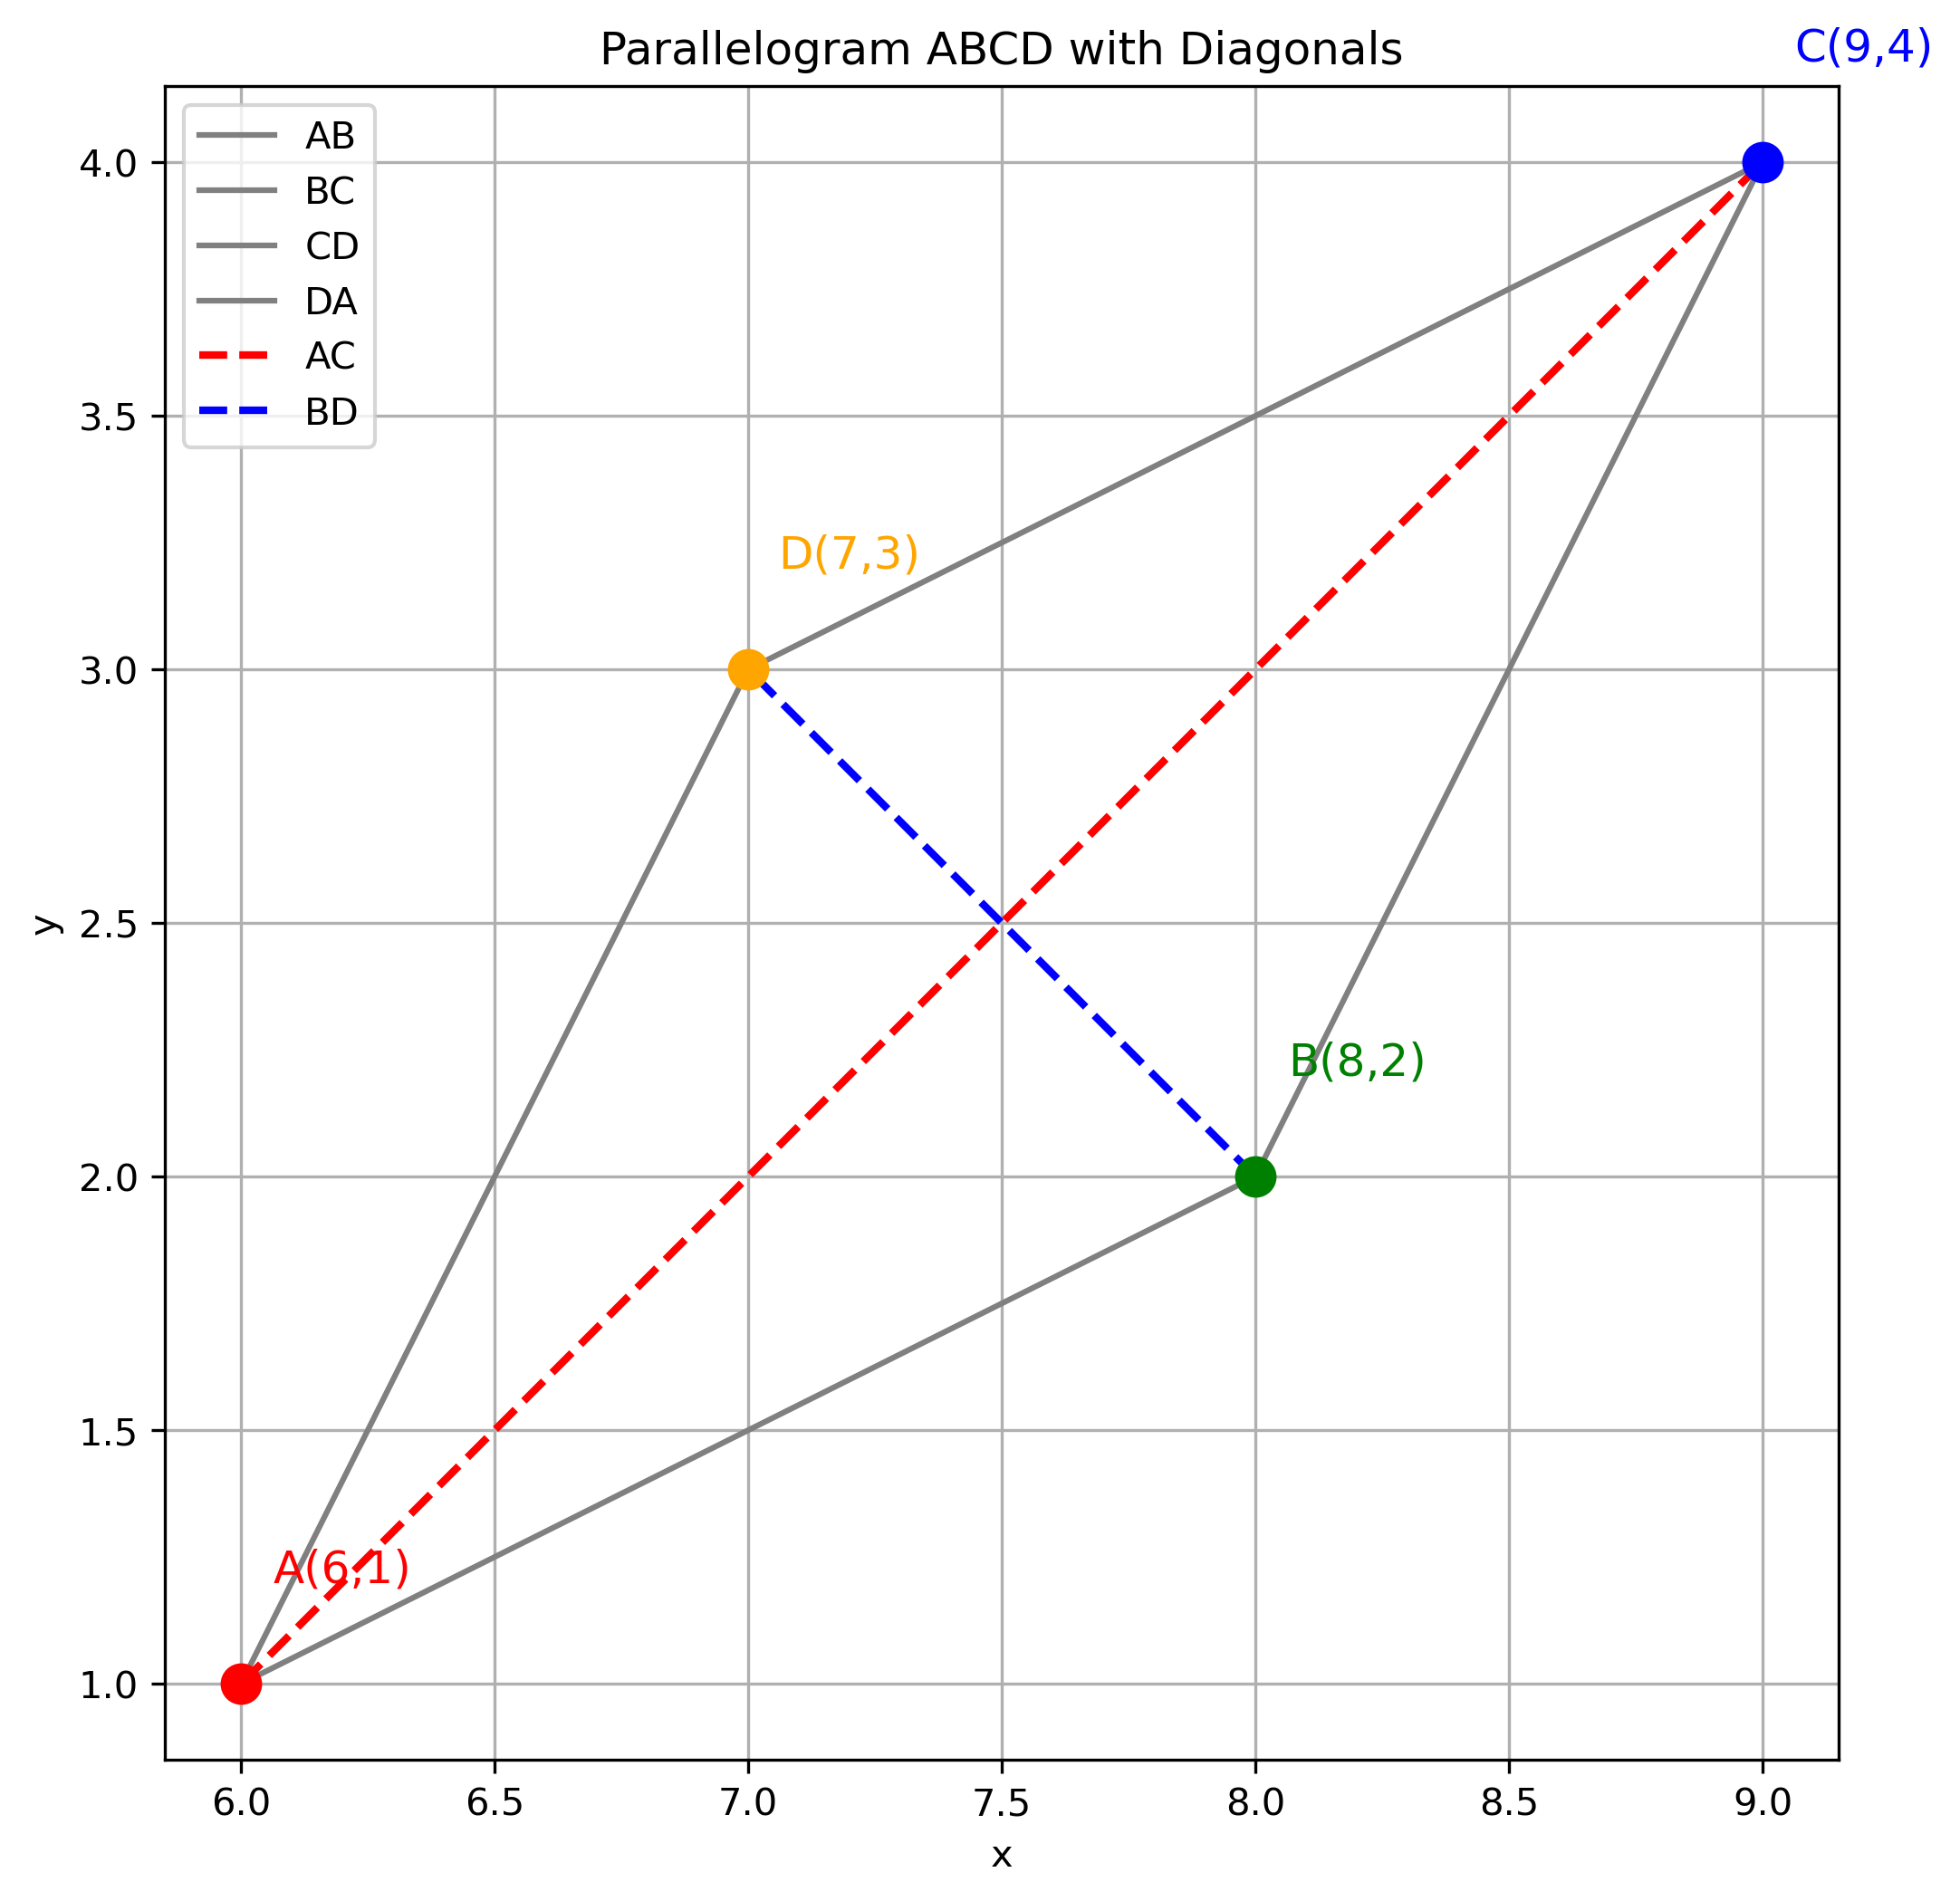
\includegraphics[width=0.5\linewidth]{figs/fig1.png}
    \caption{}
    \label{fig1}
\end{figure}
\item Identify the role of Vermiculate in vertical landscapes \hfill \textbf{(GATE EE 2025)}
\begin{enumerate}
    \begin{multicols}{2}
        \item Fertilizer
        \item Holding material
        \item Binding material
        \item Water retention element
    \end{multicols}
\end{enumerate}
\item Which of the following parameters is essential to estimate the Envelope Performance Factor(EPF) of a building as per the Energy Conservation Building Code (ECBC) ,2011? \hfill \textbf{(GATE EE 2025)}
\begin{enumerate}
    \begin{multicols}{2}
        \item Building type
        \item Maximum luminity
        \item Maximum and Minimum monthly temparature
        \item Building occupancy duration
    \end{multicols}
\end{enumerate}
\item The illumination level of a room is $300$ lux and the efficacy of the lamps is $60$.The Light Power Density (LPD) of the room in $Watt/m^2$ is \underline{\makebox[2cm]{\hfill}} \hfill \textbf{(GATE EE 2025)}\\
\item The load on a RCC column is $150\text{kN}$. The soil bearing capacity is $80 kN/m^2$. Assuming a factor of safety of $1.2$ the side of the square column footing is  \underline{\makebox[2cm]{\hfill}} meter (\textit{rounded off to one decimal place} ) \hfill \textbf{(GATE EE 2025)}\\
\item A room is separated by a partition wall.The average intensities of sound in the source and receiving sides across the partition are $10^{-4} W/m^2$ and $10^{-7} W/m^2$ respctively. The transmission loss (TL) of the partition wall is \underline{\makebox[2cm]{\hfill}} dB. \hfill \textbf{(GATE EE 2025)}\\
\item If the purchase price of 2BHK flat rises by $10\%$, the demand for such flats is observed to decrease by $8\%$ The price elasticity of the housing demand for 2BHK flats is \underline{\makebox[2cm]{\hfill}}(\textit{rounded off to one decimal place}) \hfill \textbf{(GATE EE 2025)}\\
\item Match the instruments in Column I with the various types of Surveying in column II and select the appropriate option.\hfill \textbf{(GATE EE 2025)}\\
\begin{tabular}{|c|c|c|c|} \hline
  &Column I   &   & Column II \\ \hline
 P & Cross staff    & 1 & Indoor wall to wall measurement\\ \hline
 Q & Alidabe   & 2 & Traversing\\ \hline
 R & Sextant  & 3 & Chain survey \\ \hline
 S & Distomat & 4 & Plane table survey\\ \hline
    &        & 5 & Contour survey\\ \hline
\end{tabular}
\begin{enumerate}
    \begin{multicols}{2}
        \item P-3,Q-4,R-2,S-5
        \item P-2,Q-4,R-1,S-5
        \item P-5,Q-3,R-2,S-1
        \item P-3,Q-4,R-2,S-1
    \end{multicols}
\end{enumerate}
\item Match the characteristics of settlement systems in Column I with their corresponding theory/rules in Column II and select the appropriate option.\hfill \textbf{(GATE EE 2025)}\\
\begin{tabular}{|c|c|c|c|} \hline
 & Column I & & Column II \\ \hline
P & Primacy of settlement  &1 & Central place theory  \\ \hline
Q & Settlement size and location & 2 & Gravity Model\\ \hline
R & Random component in location of settlements & 3 & Rank size rule\\ \hline
S & Interaction between settlements & 4 & Entropy of settlements\\ \hline
 & & 5 & Core Periphery model\\ \hline
\end{tabular}
\begin{enumerate}
    \begin{multicols}{2}
        \item P-4,Q-1,R-2,S-5
        \item P-2,Q-5,R-3,S-1
        \item P-3,Q-5,R-4,S-2
        \item P-3,Q-1,R-4,S-2 
    \end{multicols}
\end{enumerate}
\item Match the architectural projects in Column I with the architect in Column II and select the appropriate option. \hfill \textbf{(GATE EE 2025)}\\
\begin{tabular}{|c|c|c|c|} \hline
  & Column I &  & Column II  \\ \hline
P & India Habitat Centre,New Delhi & 1 & Christopher Charles Benninger\\ \hline
Q & United World Colleges(UWC). Mahindra College,Pune & 2 & Charles Correa\\ \hline
R & Brain \& Cognitive Science Centre-MIT,Cambrigde & 3 & Joseph Allen Stein\\ \hline
S & Habitat 67,Montreal & 4 & Norman Foster \\ \hline
 & & 5&Moshe Safdi\\ \hline 
\end{tabular}
\begin{enumerate}
    \begin{multicols}{2}
        \item P-3,Q-1,R-2,S-5
        \item P-1,Q-2,R-5,S-3
        \item P-2,Q-1,R-5,S-4
        \item P-3,Q-4,R-1,S-5
    \end{multicols}
\end{enumerate}
\item Match the Name of the book provided in Column I with the corresponding author in Column II and select the appropriate option \hfill \textbf{(GATE EE 2025)}\\
\begin{tabular}{|c|c|c|c|} \hline
 & Column I & &Column II\\ \hline
P & Earthscape &1&Ian McHarg\\ \hline
Q &Synthesis of Form &2&John O Simonds\\ \hline
R &Design with Nature&3&Christopher Alexander\\ \hline
S & The City of Tomorrow and its Planning &4&Lewis Mumford\\ \hline
 & &5&Le Corbusier\\ \hline
 \end{tabular}
 \begin{enumerate}
     \begin{multicols}{4}
        \item P-2,Q-3,R-1,S-5
         \item P-5,Q-2,R-3,S-4
         \item P-5,Q-3,R-1,S-4
         \item P-2,Q-1,R-4,S-5
     \end{multicols}
 \end{enumerate}
 \item Match the thermal properties in the Column I and their respective units in Column II and select the appropriate option \hfill \textbf{(GATE EE 2025)}\\
 \begin{tabular}{|c|c|c|c|} \hline
  & Column I &  & Column II \\ \hline
P & Thermal Resistance&1& $J kg^{-1}$$ ^\circ\text{C}^{-1}$\\ \hline
 Q &Thermal Transmittance&2&$W m^{-1}$$^\circ\text{C}^{-1}$\\ \hline 
 R & Specific Heat &3& $W m^{-2}$$^\circ\textbf{C}^{-1}$\\ \hline
 S & Thermal Conductivity &4 & $m^2$ $^\circ{C}$$W^{-1}$ \\ \hline
  & & 5 & $J m^{-3}$ $^\circ\text{C}^{-1}$\\ \hline
 \end{tabular}
 \begin{enumerate}
     \begin{multicols}{2}
         \item P-4,Q-1,R-5,S-2
         \item P-4,Q-3,R-1,S-2
         \item P-5,Q-3,R-1,S-4
         \item P-3,Q-4,R-2,S-1
     \end{multicols}
 \end{enumerate}
 \item Match the application in the field of construction in the Column I and the respective items in Column II and select the appropriate option. \hfill \textbf{(GATE EE 2025)} \\
 \begin{tabular}{|c|c|c|c|} \hline
  & Column I & & Column II \\ \hline
P &Polytetrafluoroethylene(PTFE) membrane &1 &Tendon  \\ \hline
 Q&Isolated compression component inside a network of continuous tensile member&2&TMT\\ \hline
 R&Cable used for pre-stressed concreting &3&Tensegrity\\ \hline
 S&Reinforcement bar used in RCC construction&4&TMD\\ \hline
    & &5&Teflon\\ \hline
 \end{tabular}
 \begin{enumerate}
     \begin{multicols}{2}
         \item P-5,Q-1,R-4,S-3
         \item P-4,Q-3,R-1,S-5
         \item P-5,Q-3,R-1,S-2
         \item P-3,Q-4,R-2,S-1
     \end{multicols}
 \end{enumerate}
 \item Match the following types of masonry joints in Column I with their corresponding description in Column II and select the appropriate option. \hfill \textbf{(GATE EE 2025)}\\
 \begin{figure}[H]
     \centering
     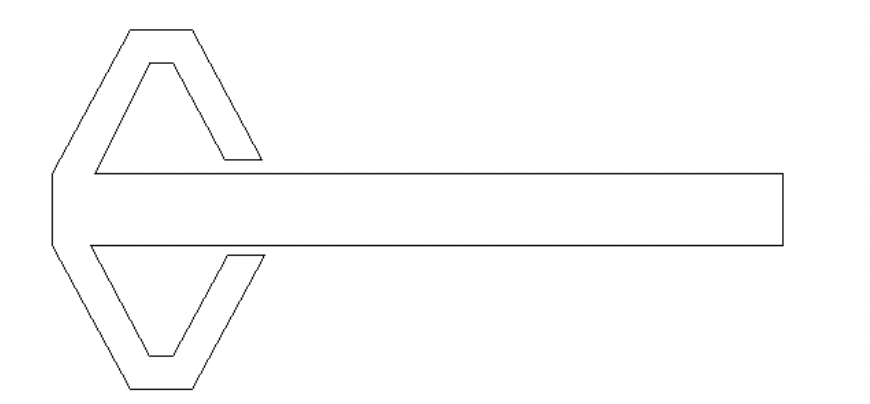
\includegraphics[width=0.5\linewidth]{figs/fig2.png}
     \caption{}
     \label{fig2}
 \end{figure}
 \begin{enumerate}
     \begin{multicols}{2}
         \item P-1,Q-3,-2,S-4
         \item P-4,Q-3,R-2,S-5
         \item P-3,Q-4,R-5,S-2
         \item P-4,Q-3,R-1,S-5
     \end{multicols}
 \end{enumerate}
 \item Match the following in Column I with their suitable descriptions in Column II and select the appropriate option.\hfill \textbf{(GATE EE 2025)}\\
 \begin{tabular}{|c|c|c|c|} \hline
  & Column I & & Column II \\ \hline
P &Tolerance &1 & $100\text{mm}$  \\ \hline
Q &Precast concrete rings for wells &2 &Non modular dimension \\ \hline
R & M & 3 & Acceptable variation\\ \hline
S & Weather joints &4 &3D-prefabricate\\ \hline
 &  & 5 & Resilient sealants\\ \hline
 \end{tabular}
 \begin{enumerate}
     \begin{multicols}{2}
         \item P-2,Q-4,R-1,S-3
         \item P-2,Q-4,R-3,S-5
         \item P-1,Q-2,R-3,S-4
         \item P-3,Q-4,R-1,S-5
     \end{multicols}
 \end{enumerate}
 \item Match the units provided in Column I with their corresponding items in Group II and select the appropriate option. \hfill \textbf{(GATE EE 2025)}\\
 \begin{tabular}{|c|c|c|c|} \hline
  & Column I & & Column II \\ \hline
P &dB&1 & Sound Intensity  \\ \hline
 Q &Phon&2&Absorption of sound\\ \hline
 R &$W/m^2$ & 3&Frequency of sound\\ \hline
 S&Sabine &4 &Loudness\\ \hline
  &   & 5 & Sound pressure level\\ \hline
 \end{tabular}
 \begin{enumerate}
     \begin{multicols}{2}
         \item P-5,Q-1,R-4,S-3
         \item P-2,Q-3,R-4,S-5
         \item P-1,Q-2,R-3,S-4
         \item P-5,Q-4,R-1,S-2
     \end{multicols}
 \end{enumerate}
 \item Match the scientific names of the trees provided in Column I with their corresponding color of their bloom in Column II and select the appropriate option \hfill \textbf{(GATE EE 2025)}
 \begin{tabular}{|c|c|c|c|} \hline
  & Column I & & Column II \\ \hline
  P&\textit{Cassia fistula}&1&White  \\ \hline
  Q&\textit{Lagerstroemia flos-reginae}&2 &Red\\ \hline
  R&\textit{Cordia sebastena} &3&Blue\\ \hline
  S&\textit{Plumeria alba}&4&Yellow\\ \hline
   &  &5&Mauve\\ \hline
 \end{tabular}
 \begin{enumerate}
     \begin{multicols}{2}
         \item P-4,Q-5,R-4,S-1
         \item P-1,Q-5,R-2,S-3
         \item P-5,Q-4,R-1,S-3
         \item P-4,Q-5,R-2,S-1
     \end{multicols}
 \end{enumerate}
 \item Match the items in Column I and their respective location in building/site in Column II and select the appropriate option \hfill \textbf{(GATE EE 2025)}\\
 \begin{tabular}{|c|c|c|c|} \hline
   & Column I &  & Column II\\ \hline
P&Nahani Trap &1&Between waste water pipe and main house drain\\ \hline
Q &Gully Trap&2&Between septic tank and soak pit\\ \hline
R&Bottle Trap &3&Junction of house drain and sewer\\ \hline
S&Intercepting Trap &4&Bathroom and Kitchen floor\\ \hline
      &  &5 &Below the wash basin\\ \hline 
 \end{tabular}
 \begin{enumerate}
     \begin{multicols}{2}
         \item P-4,Q-5,R-2,S-3
         \item P-5,Q-1,R-3,S-2
         \item P-4,Q-1,R-5,S-3
         \item P-3,Q-4,R-5,S-2
     \end{multicols}
 \end{enumerate}
 \item As per the Handbook on Barrier Free and Accessibility, CPWD - 2014, match the design guidelines in Column I with their appropriate  standards in Column II and select the appropriate option \hfill \textbf{(GATE EE 2025)}\\
 \begin{tabular}{|c|c|c|c|} \hline
  & Column I &  &  Column II \\ \hline
P &Minimum clear width of ramp&1 &$600\text{mm}$  \\ \hline
Q &Maximum height of wash basin (rim) above finished floor level &2&$1500\text{mm}$ \\ \hline
R&Minimum length of grab rail &3&$750\text{mm}$\\ \hline
 S&Minimum clear width for maneuvering space(wheelchair) & 4&$900\text{mm}$ \\ \hline
    &    & 5 & $1800\text{mm}$\\ \hline
 \end{tabular}
 \begin{enumerate}
     \begin{multicols}{2}
         \item P-3,Q-4,R-1,S-5
         \item P-5,Q-3,R-2,S-4
         \item P-5,Q-3,R-1,S-2
         \item P-1,Q-4,R-3,S-1
     \end{multicols}
 \end{enumerate}
 \item Match the contemporary Urban Design Movements listed in Column I with the corresponding principles listed in Column II. and select the appropriate option \hfill \textbf{(GATE EE 2025)}
 \begin{tabular}{|c|c|c|c|}\hline
  & Column I &  & Column II \\ \hline
P & Park Movement&1&Self-contained,self-sufficient community surrounded by green belts  \\ \hline
Q&New Urbanism&2&Revival of the relationship between man and nature\\ \hline
R&City Beautiful Movement &3&Relationship between work and living,environmental sustainability\\ \hline
S&Garden City and New Town Movement &4&Unity,cohesion and balanced relationship between urban components and elements\\ \hline
  &    & 5& Technical and socio economic processes resulting in growth,energy production and waste elimination\\ \hline
 \end{tabular}
 \begin{enumerate}
     \begin{multicols}{2}
         \item P-2,Q-3,R-4,S-1
         \item P-1,Q-5,R-3,S-2
         \item P-5,Q-3,R-1,S-2
         \item P-2,Q-5,R-4,S-1
     \end{multicols}
 \end{enumerate}
 \item Match the figures of vaults in Column I with their corresponding types in Column II and select the appropriate option.\hfill \textbf{(GATE EE 2025)}\\
 \begin{figure}[h]
     \centering
     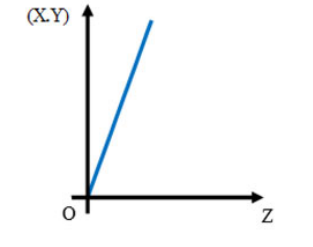
\includegraphics[width=0.5\linewidth]{figs/fig3.png}
     \caption{}
     \label{fig3}
 \end{figure}
 \begin{enumerate}
     \begin{multicols}{2}
         \item P-3,Q-4,R-1,S-2
         \item P-3,Q-1,R-4,S-5
         \item P-2,Q-1,R-5,S-3
         \item P-2,Q-3,R-1,S-5
     \end{multicols}
 \end{enumerate}
 \item Match the figures of vaults in Column I with their corresponding types in Column II and select the appropriate option \hfill \textbf{(GATE EE 2025)}\\
 \begin{enumerate}
     \begin{multicols}{2}
         \item P-3,Q-4,R-1,S-2
         \item P-3,Q-1,R-4,S-5
         \item P-2,Q-1,R-5,S-3
         \item P-2,Q-3,R-1,S-5
     \end{multicols}
 \end{enumerate}
 \item A colony of 50 people is served by a septic tank.The rate of water supply is $90\text{lcpd}$ in the colony and $40\%$ of it is going to the septi tank. The retention period of the tank is 24 hours. The retention period of the tank is 24 hours. The length of the specific tank is \underline{\makebox[2cm]{\hfill}} meter(\textit{rounded off to two decimal places}).\hfill \textbf{(GATE EE 2025)}\\
 Assume,Storage capacity/person=$0.085 m^3$ (3 years)\\
 space for digestion=$0.0425 m^3/person$\\
 Depth of tank=1.4 m\\
 $Length:width$ =$2:1$\\
 \item A cone with a base 10 cm diameter and axis of 12 cm is lying on Horizontal plane (HP) along its generator. The internal angle which the base of the cone makes with the HP is \underline{\makebox[2cm]{\hfill}} degrees. \hfill \textbf{(GATE EE 2025)}\\
 \item A public utility building of $5000$ ${m^2}$ was constucted 5 years before, on a site of $1 hectare$ The present value of open land in that location is Rs. $100/m^2$ and present construction cost of such building is Rs. $2500/m^2$. If the value of the building is assumed to be depreciation at a constant rate of $6\%$ per annum, Then the present value of the property using 'Valuation by Cost Method' is \underline{\makebox[2cm]{\hfill}} (in Rs. lakhs) (\textit{rounded off to one decimal place}).\hfill \textbf{(GATE EE 2025)}\\
 \item A residential area of 20 hectares is planned for three different types of plots of $500$ ${m^2}$ ,$300$ $m^2$ and $200$ $m^2$ with numbers of plot in each category are 100,120 and 150 respectively. The rest of the area is allocated for roads and facilities such as schools ,shops and parks. The net residential density of the area in persons per hectare is \underline{\makebox[2cm]{\hfill}}. \hfill \textbf{(GATE EE 2025)}
 \item In a single lane road, traffic volume of 1000 $vehicle/h$ moving at 20 $km/h$, comes to a halt due to an accident .If  jam density is 150 $vehicle/km$ ,the velocity of the shock wave generated (in absolute value) is \underline{\makebox[2cm]{\hfill}} $km/hr$ \hfill \textbf{(GATE EE 2025)}
 \item In a site map, a rectangular residential plot measures $150\text{mm} \quad \times 40\text{mm}$ ,and the width of the front road in the map measures 16 mm. Actual width of the road is 4m. If the permissible F.A.R. is $1.2$ ,The maximum built-up area for the residential building will be \underline{\makebox[2cm]{\hfill}} $m^2$. \hfill \textbf{(GATE EE 2025)}
\item The internal dimension of a room is $10 \text{m} \times 10  \text{m} \times 4 \text{m}$ (height).  
The total area of the doors and windows are $16 \, \text{m}^2$. Keeping the doors and windows closed, 
the reverberation time of the room becomes $1.2 \, \text{seconds}$.  
Assume all the interior surfaces including doors and windows have the same sound absorption coefficient.  
If all the doors and windows of the room are kept fully open, the reverberation time will be 
\underline{\makebox[2cm]{\hfill}} seconds (rounded off to two decimal places). \hfill \textbf{(GATE EE 2025)}

\item A depressed portion of a land is identified by three closed contours, as shown in the figure below.  
The area bounded by three contour lines are $6  \text{m}^2$, $24  \text{m}^2$ and $96  \text{m}^2$ respectively.  
\begin{figure}[H]
    \centering
    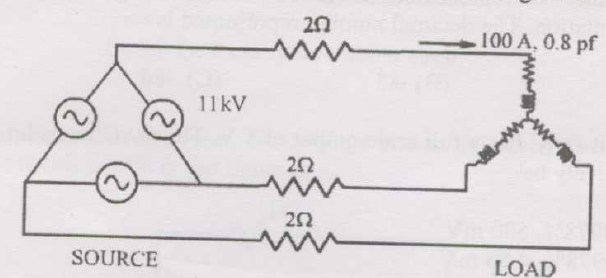
\includegraphics[width=0.5\linewidth]{figs/fig4.png}
    \caption{}
    \label{fig4}
\end{figure}
The contour interval is 1 m. Using prismoidal method, the volume of the earth needed to fill the land depression is \underline{\makebox[2cm]{\hfill}} $\text{m}^3$. \hfill \textbf{(GATE EE 2025)}
\item Solar panels are proposed to be installed on a building roof top to generate electricity.  
The size of each solar panel is $2 \, \text{m}^2$. The efficiency of each panel is $75\%$.  
The orientations of the solar panel and related solar data are given in the table below:\hfill \textbf{(GATE EE 2025)}\\
\begin{tabular}{|c|c|c|c|}\hline
\text{Orientation} & \text{No. of Panels} & 
\text{Average Daily Solar Radiation $(W/m^2)$} & 
\text{Average Solar Hours per Day} \\ \hline
\text{South} & 10 & 400 & 4 \\ \hline
\text{West} & 5 & 300 & 2 \\ \hline
\end{tabular}
As per the above proposal, \underline{\makebox[2cm]{\hfill}} kWh solar power will be generated daily  
(\textit{rounded off to one decimal place}). \hfill \textbf{(GATE EE 2025)}\\
\item A power shovel is having $1.8 \, \text{m}^3$ excavation output per batch of operation.  
The average cycle time of the batch operation is $45$ seconds. The lost time per hour of the excavation activity is $10$ minutes.  
Assume six working hours of operation per day. The amount of soil excavated by the power shovel per day is 
\underline{\makebox[2cm]{\hfill}} $\text{m}^3$ (rounded off to two decimal places). \hfill \textbf{(GATE EE 2025)}\\

\item A room having dimension $12 \, m \times 10 \, m \times 3.5 \, m$ is required to be mechanically ventilated by air-conditioner. The temperature difference between outdoor ambient air and the supply air is $12^\circ C$. Consider three air exchanges per hour. The volumetric specific heat of the air is $1250 \, J/m^3{}^\circ C$. Assume one ton of refrigeration (TR) is equal to $3.5 \, kW$. The capacity of the air-conditioner for the room in TR will be \underline{\makebox[2cm]{\hfill}}.\hfill \textbf{(GATE EE 2025)} \\
\item A simply supported beam AB has a clear span of 7 meter. The bending moment diagram (BMD) of the beam due to a single concentrated load is shown in the figure below. \\
\begin{figure}[H]
    \centering
    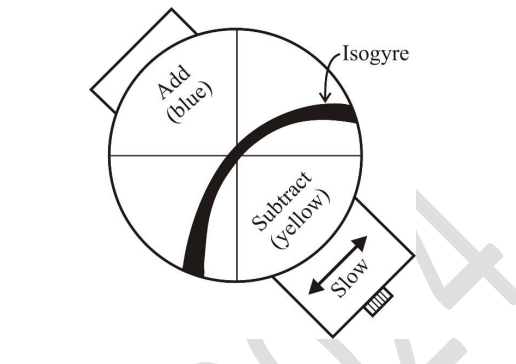
\includegraphics[width=0.5\linewidth]{figs/fig5.png}
    \caption{}
    \label{fig5}
\end{figure}
The magnitude of the concentrated load in kN is \underline{\makebox[2cm]{\hfill}}.\hfill \textbf{(GATE EE 2025)} \\

\item For a symmetrical trapezoidal open drain in a landscape with grass and loose rock surface, the velocity of flow of water is \underline{\makebox[2cm]{\hfill}} m/sec, (rounded off to two decimal places), given the following data.\hfill \textbf{(GATE EE 2025)} \\

\begin{tabular}{ll}
Water edge width at the top &= 750 mm \\
Water edge width at the bottom &= 450 mm \\
Water depth &= 600 mm \\
Manning's coefficient of roughness &= $0.05$ \\
Slope along the drain &= 1 in 250 \\
\end{tabular} \\
\item The stack pressure is created by 10 m height of stack and $15^\circ C$ temperature difference. The motive force due to the stack pressure over a cross section area of $2.5 \, m^2$ is \underline{\makebox[2cm]{\hfill}} N.\hfill \textbf{(GATE EE 2025)} \\


\item An industrial building contains 3000 kg of combustible materials, in dry state, distributed over three rooms of area $100 \, m^2$, $500 \, m^2$ and $300 \, m^2$ each, in a proportion of 30\%, 50\% and 20\% of the contents, respectively. Calorific value of the material is $4400 \, kCal/kg$. The Total Fire Load of the rooms is equal to \underline{\makebox[2cm]{\hfill}} kCal/m$^2$. \hfill \textbf{(GATE EE 2025)}\\
\item A simple truss is shown in the figure below. The truss is loaded with horizontal and vertical force $15 \, kN$ and $25 \, kN$, respectively. The force in the member AB will be \underline{\makebox[2cm]{\hfill}} kN. \hfill \textbf{(GATE EE 2025)} \\
\begin{figure}[H]
    \centering
    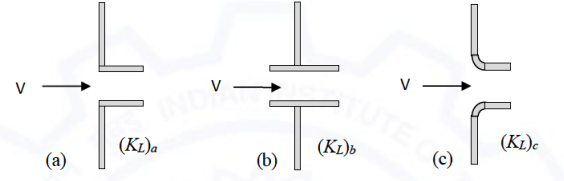
\includegraphics[width=0.5\linewidth]{figs/fig6.png}
    \caption{}
    \label{fig6}
\end{figure}
\end{enumerate}
\end{document}
